\section{Infrastructure}
\subsection{Domain information}

Here we work our way piece by piece {\bf from rough to detailed} information.
Therefore we first have to get a technical overview of the company. Since we
usually already know the name of the company or even the domain name, this
information is generally sufficient to determine how the company is
structured.
\begin{figure}
  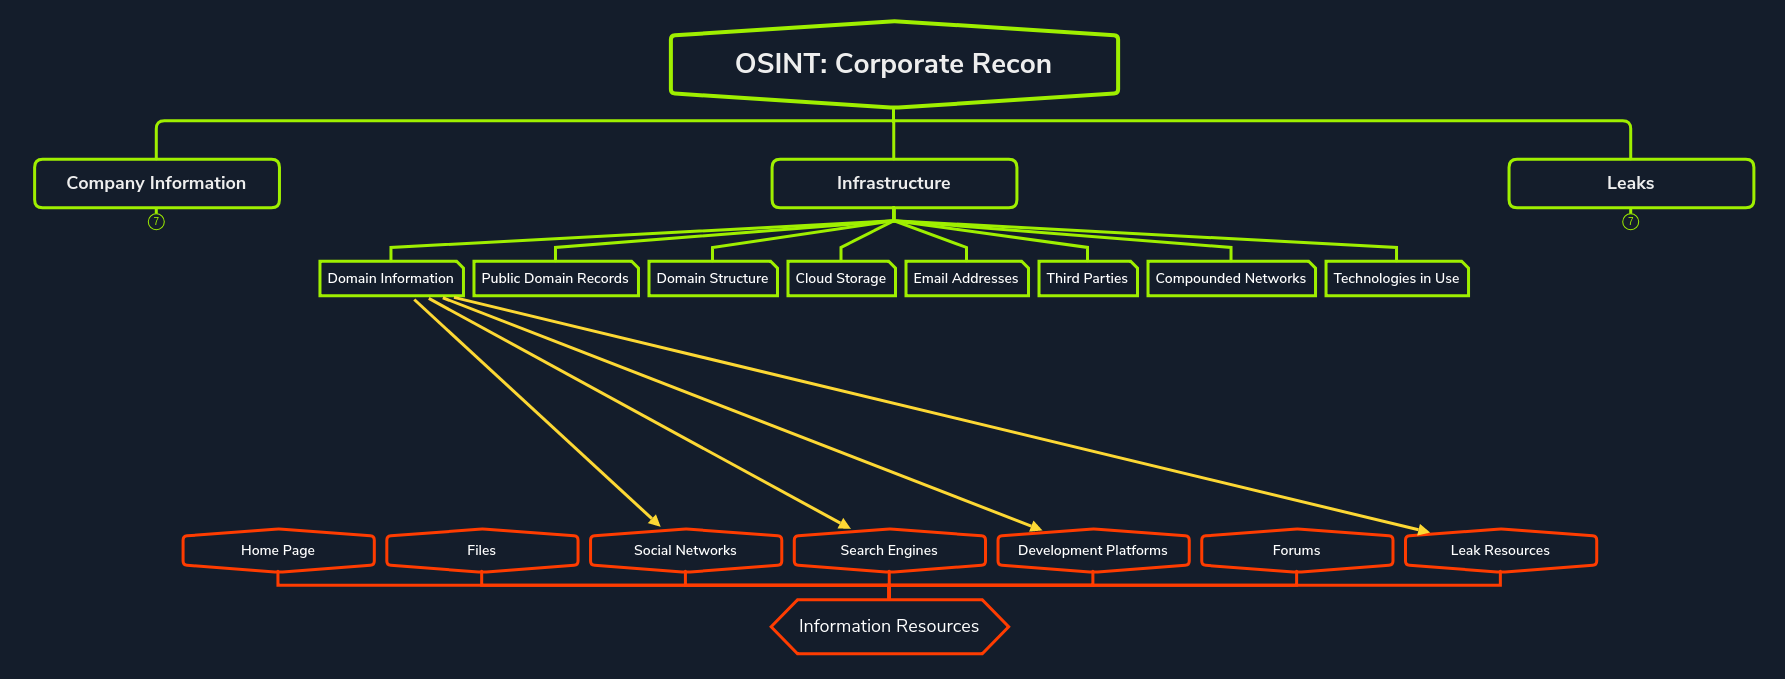
\includegraphics[width=\linewidth]{recon/osint/images/infra-domain-info.png}
  \caption{OSINT Domain information}
  \label{fig:osint-domain-info}
\end{figure}

The element we focus on in the first phase of the company's infrastructure
investigation is the domain names we can find. We then go into each domain and
get an overview of the subordinate structure that contains 
\begin{itemize}
        \item Netblocks
        \item Name Servers
        \item Mail Servers
        \item subdomains
        \item hosts/IP addresses.
\end{itemize}

We can classify the rough structure into three categories:
\begin{itemize}
        \item Public Records:  	
        \item Third Parties 	
        \item Domains
\end{itemize}

\subsubsection{Social Networks}
We often find references to domains or subdomains on social media platforms.


\subsubsection{Search Engines}
One of the most efficient methods of searching for domains is offered by
various search engines. In this case, we cannot focus on a domain name, but we
have to work with general company terms, such as the company name, the name of
the application or service, and others.

Another excellent way to find out information about our target domain is to use
a particular Search Engine Optimization (SEO) field called backlinks. 

One of such backlinks analyzers is
\href{https://app.neilpatel.com/en/seo_analyzer/backlinks}{Ubersuggest}.

\subsubsection{Development Platforms}
Development platforms also offer excellent information resources for us here,
as we will often find code that sometimes even provide information that is
dangerous for the company. This information can range from IP addresses and
hostnames, configuration files to credentials.

\subsubsection{Leak Resources}
Once we have a list of the company's domains, we can use it to look for known
anomalies that affect the company and the corresponding domain. One of the best
sources of information for this is
\href{https://www.virustotal.com/}{VirusTotal}, where we can scan each domain
for suspicious activity.


Another source that searches against many different developer platforms is
\href{https://searchcode.com/}{Searchcode}. It searches all possible codes for
terms that we specify in the search and shows us the sources accordingly.

\section{Public Domain Records}

Public domain records offer us excellent opportunities to trace the company's
information technology infrastructure structure. With the right arrangement and
knowledge of what the records are for and what information they contain, they
can provide us with information about the company's Internet presence. To get
this, we need to find out at least four components:
\begin{verbatim}
1. Netblocks / CIDR 	2. ASN 	3. DNS Servers 	4. Mail Servers
\end{verbatim}

This gives us an overview of which systems are accessible from the internet, in
which address range they are located, which IP neighbors they have, and how the
interaction between them takes place.

\begin{figure}
  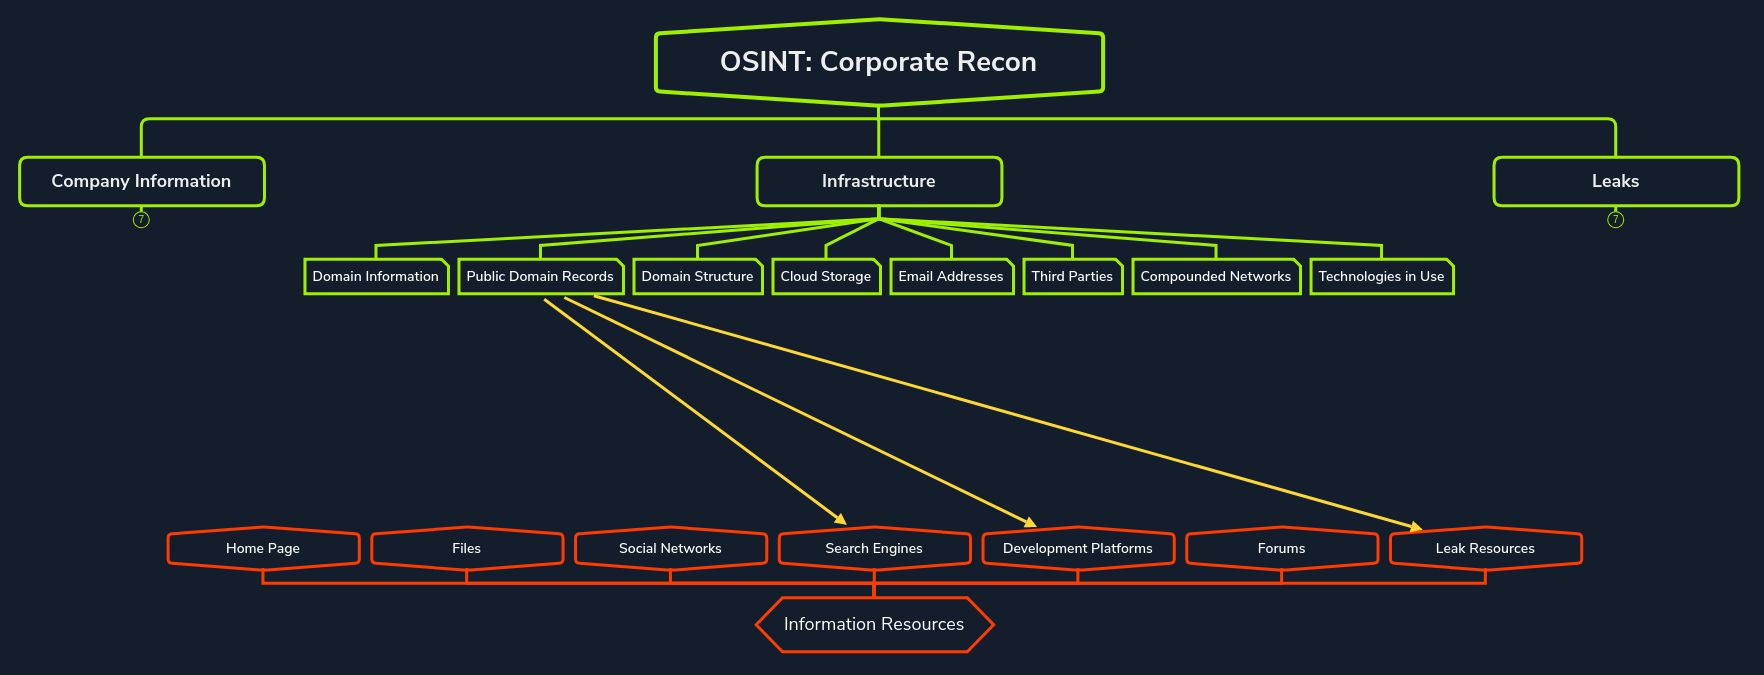
\includegraphics[width=\linewidth]{recon/osint/images/infra-pub-records.png}
  \caption{OSINT Domain public records}
  \label{fig:osint-infra-pub-records}
\end{figure}

